\documentclass[german,10pt]{book}      
\usepackage{makeidx}
\usepackage{babel}            % Sprachunterstuetzung
\usepackage{amsmath}          % AMS "Grundpaket"
\usepackage{amssymb,amsfonts,amsthm,amscd} 
\usepackage{mathrsfs}
\usepackage{rotating}
\usepackage{sidecap}
\usepackage{graphicx}
\usepackage{color}
\usepackage{fancybox}
\usepackage{tikz}
\usetikzlibrary{arrows,snakes,backgrounds}
\usepackage{hyperref}
\hypersetup{colorlinks=true,
                    linkcolor=blue,
                    filecolor=magenta,
                    urlcolor=cyan,
                    pdftitle={Overleaf Example},
                    pdfpagemode=FullScreen,}
%\newcommand{\hyperref}[1]{\ref{#1}}
%
\definecolor{Gray}{gray}{0.80}
\DeclareMathSymbol{,}{\mathord}{letters}{"3B}
%
\newcounter{num}
\renewcommand{\thenum}{\arabic{num}}
\newenvironment{anmerkungen}
   {\begin{list}{(\thenum)}{%
   \usecounter{num}%
   \leftmargin0pt
   \itemindent5pt
   \topsep0pt
   \labelwidth0pt}%
   }{\end{list}}
%
\renewcommand{\arraystretch}{1.15}                % in Formeln und Tabellen   
\renewcommand{\baselinestretch}{1.15}                 % 1.15 facher
                                                      % Zeilenabst.
\newcommand{\Anmerkung}[1]{{\begin{footnotesize}#1 \end{footnotesize}}\\[0.2cm]}
\newcommand{\comment}[1]{}
\setlength{\parindent}{0em}           % Nicht einruecken am Anfang der Zeile 

\setlength{\textwidth}{15.4cm}
\setlength{\textheight}{23.0cm}
\setlength{\oddsidemargin}{1.0mm} 
\setlength{\evensidemargin}{-6.5mm}
\setlength{\topmargin}{-10mm} 
\setlength{\headheight}{0mm}
\newcommand{\identity}{{\bf 1}}
%
\newcommand{\vs}{\vspace{0.3cm}}
\newcommand{\noi}{\noindent}
\newcommand{\leer}{}

\newcommand{\engl}[1]{[\textit{#1}]}
\parindent 1.2cm
\sloppy

         \begin{document}  \setcounter{chapter}{2}

%\newcommand{\solution}[1]{}

\chapter{Entropie -- Statistische Zug\"ange}
% Kap x
\label{chap_Entropie}

Wir unterscheiden
mindestens drei verschiedene Entropiebegriffe: (1) die thermodynamische Entropie, die
mit einem Fluss an W\"armeenergie verbunden ist, (2) die Boltzmann-Entropie der statistischen
Mechanik und (3) die Shannon-Entropie der Informationstheorie. Der thermodynamische
Entropiebegriff wird in einen anderen Kurztext behandelt (siehe \glqq \hyperref[chapter_ZweiteHS]{Der zweite
Hauptsatz der Thermodynamik}\grqq).
In diesem Kurztext geht es im Wesentlichen um die Shannon-Entropie, die man als 
\glqq Ma\ss\ f\"ur Unkenntnis\grqq\ interpretieren kann, sowie der Boltzmann-Entropie, 
die als \glqq Ma\ss\ f\"ur Unordnung\grqq\ gedeutet werden kann.

Schwieriger ist der Beweis, dass diese beiden Definitionen von Entropie \"aquivalent
zum thermodynamischen Entropiebegriff sind. Auch Boltzmann hat dies zun\"achst nur
f\"ur das ideale Gas gezeigt. Diese \"Aquivalenz soll auch hier bewiesen werden. 

\section{Die Shannon-Information}
\label{sec_Shannon}

Im Jahre 1948 ver\"offentlichte Claude Elwood Shannon (1916--2001) sein Hauptwerk {\em A Mathematical Theory
of Communication} \cite{Shannon} 
und formulierte dort ein Ma\ss\ f\"ur Information (heute als {\em Shannon-Information} bekannt). 
Bald darauf wurde der Bezug dieser Gr\"o\ss e zum Entropiebegriff in der statistischen Mechanik deutlich. 
Shannon ging es haupts\"achlich um ein Ma\ss\ f\"ur den Verlust an Information, der durch fehlerhafte 
Signal\"ubertragung bei Kommunikationssystemen auftritt. 

\subsection{Die Shannon-Information als fehlende Information}

Wir stellen uns ein System vor, das viele verschiedene Zust\"ande annehmen kann. 
Mit $\Omega$ bezeichnen wir die Menge dieser Zust\"ande und $\{p_i\}$ sei eine Wahrscheinlichkeitsverteilung,
die angibt, mit welcher Wahrscheinlichkeit $p_i$ ein bestimmter Zustand $i \in \Omega$ vorliegt. Statt Zustand
schreibe ich manchmal auch Mikrozustand oder Ereignis, wobei hier eigentlich ein Elementarereignis gemeint
ist. Wir fragen nun nach einem Ma\ss\ f\"ur die \textit{fehlende Information}, um aus der Kenntnis
der Wahrscheinlichkeiten $\{ p_i \}$ auf einen ganz bestimmten realisierten Zustand schlie\ss en zu k\"onnen.

Als Einheit der Information gilt das Bit, dessen beide Werte 1 oder 0 bzw.\ TRUE oder FALSE sein k\"onnen. 
Als Ma\ss\ f\"ur die fehlende Information w\"ahlen wir die minimale Anzahl von
Bits (gemessen durch die Antworten auf Ja/Nein-Fragen), mit denen wir die 
gew\"unschte Information erlangen. Konkret: Wie viele
Ja/Nein-Fragen m\"ussen wir im Mittel mindestens stellen und beantwortet bekommen, um von der 
allgemeinen Information \"uber die Wahrscheinlichkeitsverteilung zu der Information der 
speziellen Realisierung zu gelangen? 

Wir betrachten zun\"achst als Beispiel ein Schachbrett mit 64 Feldern. Die allgemeine Information
sei: Auf einem Feld des Schachbretts befindet sich eine Figur. Diese Information umfasst die Menge der
M\"oglichkeiten $\Omega$ (64 Felder) sowie die Wahrscheinlichkeitsverteilung, in diesem Fall die 
Gleichverteilung: $p_i=1/64$. Gesucht ist das konkrete Feld, auf dem sich die Figur
befindet. Wir k\"onnen nat\"urlich alle Felder einzeln erfragen: Steht die Figur auf Feld 1? Steht sie auf
Feld 2? etc. Im Durchschnitt w\"urden wir in diesem Fall 32 Fragen ben\"otigen, bis das besetzte 
Feld bekannt ist.

Bei geschickter Wahl der Fragen ben\"otigen wir jedoch genau 6 Ja/Nein-Fragen, um das Feld zu finden.
Dazu unterteilen wir die M\"oglichkeiten immer in zwei m\"oglichst gleichwahrscheinliche Bereiche (siehe
Abb.\ \ref{fig_Schachbrett}). 
Die erste Frage k\"onne lauten: Befindet sich die Figur auf der linken Spielfeldh\"alfte? 
Die zweite Frage w\"are beispielsweise: Ist die Figur in der oberen H\"alfte? usw. Da sich mit
jeder beantworteten Frage die Anzahl der M\"oglichkeiten halbiert, ist das gesuchte Feld nach sechs 
Fragen gefunden. Wir k\"onnen also sagen: Die fehlende Information zwischen der Situation, wo
man nur wei\ss, dass sich auf einem Feld des Spielfelds eine Figur befindet, bis zu der Kenntnis,
um welches Feld es sich dabei genau handelt, betr\"agt 6 Bits. 

\begin{figure}[htb]
\begin{picture}(70,70)(0,0)
\multiput(5,5)(0,7.5){9}{\line(1,0){60}}
\multiput(5,5)(7.5,0){9}{\line(0,1){60}}
\multiput(8.75,8.25)(7.5,0){4}{\makebox(0,0){x}}
\multiput(8.75,15.75)(7.5,0){4}{\makebox(0,0){x}}
\multiput(8.75,23.25)(7.5,0){4}{\makebox(0,0){x}}
\multiput(8.75,30.75)(7.5,0){4}{\makebox(0,0){x}}
\multiput(8.75,38.25)(7.5,0){4}{\makebox(0,0){x}}
\multiput(8.75,45.75)(7.5,0){4}{\makebox(0,0){x}}
\multiput(8.75,53.25)(7.5,0){4}{\makebox(0,0){x}}
\multiput(8.75,60.75)(7.5,0){4}{\makebox(0,0){x}}
\end{picture}
%
\begin{picture}(70,70)(0,0)
\multiput(5,5)(0,7.5){9}{\line(1,0){60}}
\multiput(5,5)(7.5,0){9}{\line(0,1){60}}
\multiput(8.75,8.25)(7.5,0){4}{\makebox(0,0){x}}
\multiput(8.75,15.75)(7.5,0){4}{\makebox(0,0){x}}
\multiput(8.75,23.25)(7.5,0){4}{\makebox(0,0){x}}
\multiput(8.75,30.75)(7.5,0){4}{\makebox(0,0){x}}
\multiput(8.75,38.25)(7.5,0){8}{\makebox(0,0){x}}
\multiput(8.75,45.75)(7.5,0){8}{\makebox(0,0){x}}
\multiput(8.75,53.25)(7.5,0){8}{\makebox(0,0){x}}
\multiput(8.75,60.75)(7.5,0){8}{\makebox(0,0){x}}
\end{picture}
%
\begin{picture}(70,70)(0,0)
\multiput(5,5)(0,7.5){9}{\line(1,0){60}}
\multiput(5,5)(7.5,0){9}{\line(0,1){60}}
\multiput(8.75,8.25)(7.5,0){8}{\makebox(0,0){x}}
\multiput(8.75,15.75)(7.5,0){8}{\makebox(0,0){x}}
\multiput(8.75,23.25)(7.5,0){4}{\makebox(0,0){x}}
\multiput(8.75,30.75)(7.5,0){4}{\makebox(0,0){x}}
\multiput(8.75,38.25)(7.5,0){8}{\makebox(0,0){x}}
\multiput(8.75,45.75)(7.5,0){8}{\makebox(0,0){x}}
\multiput(8.75,53.25)(7.5,0){8}{\makebox(0,0){x}}
\multiput(8.75,60.75)(7.5,0){8}{\makebox(0,0){x}}
\end{picture}
%
\begin{picture}(70,70)(0,0)
\multiput(5,5)(0,7.5){9}{\line(1,0){60}}
\multiput(5,5)(7.5,0){9}{\line(0,1){60}}
\multiput(8.75,8.25)(7.5,0){8}{\makebox(0,0){x}}
\multiput(8.75,15.75)(7.5,0){8}{\makebox(0,0){x}}
\multiput(8.75,23.25)(7.5,0){4}{\makebox(0,0){x}}
\multiput(53.75,23.25)(7.5,0){2}{\makebox(0,0){x}}
\multiput(8.75,30.75)(7.5,0){4}{\makebox(0,0){x}}
\multiput(53.75,30.75)(7.5,0){2}{\makebox(0,0){x}}
\multiput(8.75,38.25)(7.5,0){8}{\makebox(0,0){x}}
\multiput(8.75,45.75)(7.5,0){8}{\makebox(0,0){x}}
\multiput(8.75,53.25)(7.5,0){8}{\makebox(0,0){x}}
\multiput(8.75,60.75)(7.5,0){8}{\makebox(0,0){x}}
\end{picture}
%
\begin{picture}(70,70)(0,0)
\multiput(5,5)(0,7.5){9}{\line(1,0){60}}
\multiput(5,5)(7.5,0){9}{\line(0,1){60}}
\multiput(8.75,8.25)(7.5,0){8}{\makebox(0,0){x}}
\multiput(8.75,15.75)(7.5,0){8}{\makebox(0,0){x}}
\multiput(8.75,23.25)(7.5,0){4}{\makebox(0,0){x}}
\multiput(53.75,23.25)(7.5,0){2}{\makebox(0,0){x}}
\multiput(8.75,30.75)(7.5,0){8}{\makebox(0,0){x}}
\multiput(8.75,38.25)(7.5,0){8}{\makebox(0,0){x}}
\multiput(8.75,45.75)(7.5,0){8}{\makebox(0,0){x}}
\multiput(8.75,53.25)(7.5,0){8}{\makebox(0,0){x}}
\multiput(8.75,60.75)(7.5,0){8}{\makebox(0,0){x}}
\end{picture}
%
\begin{picture}(70,70)(0,0)
\multiput(5,5)(0,7.5){9}{\line(1,0){60}}
\multiput(5,5)(7.5,0){9}{\line(0,1){60}}
\multiput(8.75,8.25)(7.5,0){8}{\makebox(0,0){x}}
\multiput(8.75,15.75)(7.5,0){8}{\makebox(0,0){x}}
\multiput(8.75,23.25)(7.5,0){4}{\makebox(0,0){x}}
\multiput(46.25,23.25)(7.5,0){3}{\makebox(0,0){x}}
\multiput(8.75,30.75)(7.5,0){8}{\makebox(0,0){x}}
\multiput(8.75,38.25)(7.5,0){8}{\makebox(0,0){x}}
\multiput(8.75,45.75)(7.5,0){8}{\makebox(0,0){x}}
\multiput(8.75,53.25)(7.5,0){8}{\makebox(0,0){x}}
\multiput(8.75,60.75)(7.5,0){8}{\makebox(0,0){x}}
\end{picture}
\caption{\label{fig_Schachbrett}%
Nach 6 geschickt gestellten Ja/Nein-Fragen kann die Anzahl der M\"oglichkeiten von 64 auf
1 reduziert werden. Die erste Frage k\"onnte lauten: Befindet sich die Figur in der linken H\"alfte? Die Antwort
\glqq Nein\grqq\ l\"asst nur noch 32 M\"oglichkeiten zu (linkes Bild). Die zweite Frage: Befindet sich die Figur auf der
oberen H\"alfte? reduziert die Anzahl der verbliebenen M\"oglichkeiten auf 16 (zweites Bild), etc.}
\end{figure}

Mit jeder Antwort auf eine geschickt gestellte Frage verringert sich die Anzahl
der M\"oglichkeiten um die H\"alfte und damit verdoppeln sich  
die Wahrscheinlichkeiten f\"ur die verbliebenen M\"oglichkeiten.
Nachdem bei dem Schachbrett zu Beginn die Wahrscheinlichkeit f\"ur jedes Feld $1/64$ betrug,
fallen nach Beantwortung der ersten Frage 32 Felder weg und f\"ur die 32 verbliebenen Felder wird die
Wahrscheinlichkeit, dort die Figur zu finden, zu $1/32$.
Die Fragen enden, wenn nur noch ein Ereignis, das nun die Wahrscheinlichkeit 1 hat, \"ubrig bleibt. 
Nun ist der Mikrozustand bekannt. Im vorliegenden Fall muss man $6=-\log_2 (1/64)=\log_2 64$ Fragen stellen,
bis das Feld auf dem Schachbrett bekannt ist.

Allgemein ist die optimale Strategie die folgende: Sei $\Omega$ die Menge der m\"oglichen Zust\"ande und
$\{p_i\}$ die Wahrscheinlichkeitsverteilung f\"ur die einzelnen Zust\"ande $i$. Wir teilen nun $\Omega$ in zwei
disjunkte Teilmengen $A_1$ und $A_2$ auf -- also $\Omega=A_1\cup A_2$ und $A_1\cap A_2=\emptyset$ --, sodass
$p(A_1)=\sum_{i\in A_1} p_i = p(A_2)=\sum_{i\in A_2} = 1/2$. Die erste Frage lautet dann beispielsweise: Befindet sich der
gesuchte Mikrozustand in $A_1$? Lautet die Antwort \glqq Ja\grqq, fahren wir mit $A_1$ fort. Lautet die Antwort \glqq Nein\grqq,
fahren wir mit $A_2$ fort. Wir unterteilen nun die verbliebene Menge an Mikrozust\"anden wieder in zwei Teilmengen
mit jeweils einer Wahrscheinlichkeit von $1/2$ und stellen die n\"achste Frage. 

War $p_i$ die anf\"angliche Wahrscheinlichkeit f\"ur ein Ereignis $i$ und ist dieses nach $n$ Schritten der 
Ja/Nein-Auswahl noch \"ubrig, so ist dessen Wahrscheinlichkeit nach $n$ Schritten somit $2^n p_i$.
F\"ur irgendein $n_i$ an Fragen wird diese Wahrscheinlichkeit gleich 1, der Zustand $i$ liegt also mit
Sicherheit vor. Somit ist
\begin{equation}
      2^{n_i} p_i = 1 ~~~  {\rm oder} ~~~ n_i= - \log_2 p_i \, .
\end{equation} 
Das bedeutet, die Anzahl $n_i$ der notwendigen Ja/Nein-Fragen, bis ein Mikrozustand, der 
zu Beginn mit der Wahrscheinlichkeit $p_i$ vorliegt, als realisiertes Ereignis bekannt ist, 
ist $n_i=- {\rm log}_2 p_i$. 

Einem Ereignis, von dem bekannt ist, dass es mit der 
Wahrscheinlichkeit $p_i$ vorliegen kann, ordnen
wir somit die (fehlende) Information
\begin{equation}
            I_i = - {\rm log}_2 p_i 
\end{equation}
zu. Die mittlere (fehlende) 
Information zu einer Wahrscheinlichkeitsverteilung
$\{p_i\}$ ist dann
\begin{equation}
        \bar{I}[\{p_i\}] = \sum_i I_i p_i = - \sum_i p_i \, {\rm log}_2 p_i   \, .
\end{equation}
Diese Gr\"o\ss e bezeichnet man als die {\em Shannon-Information}
zu einer Verteilung $\{ p_i\}$.  

Im Allgemeinen handelt es sich hier nur um eine idealisierte untere Grenze f\"ur die mittlere
Anzahl an Ja/Nein-Fragen, die man stellen muss, bis ein Mikrozustand bekannt ist. Der Grund ist,
dass $1/p_i$ im Allgemeinen keine Potenz von $2$ ist und somit die Aufteilung einer Teilmenge
$A \subset \Omega$ in zwei Unterteilmengen, die jeweils exakt die H\"alfte der verbliebenen
Wahrscheinlichkeiten haben, meist nicht m\"oglich sein wird. Doch jedes Abweichen von dieser
Optimalstrategie erh\"oht die mittlere Anzahl der notwendigen Fragen, bis der
Mikrozustand bekannt ist.

\subsection{Die Maximierung der Shannon-Information}

Wir stellen nun die Frage, f\"ur welche Wahrscheinlichkeitsverteilung auf einer Menge $\Omega$ 
von diskreten Elementarereignissen die Shannon-Information maximal wird. Dabei setzen wir
bestimmte Informationen \"uber diese Wahrscheinlichkeiten voraus. In diesem Zusammenhang ist
es oft einfacher (und n\"aher an den in der Physik verwendeten Gr\"o\ss en), wenn man nicht
den Logarithmus zur Basis 2 sondern den nat\"urlichen Logarithmus verwendet. Wegen
\begin{equation}
              \log_2 x =  (\log_2 {\rm e}) \,   \ln x  \hspace{1cm} {\rm bzw.} \hspace{1cm}
              \ln x = (\ln 2) \, \log_2 x
\end{equation}
sind die beiden Funktionen proportional zueinander und die Extremalpunkte sind dieselben. 

\subsubsection{Die Gleichverteilung}

Wir beginnen mit der Suche nach einer Wahrscheinlichkeitsverteilung, welche die
Shannon-Information maximiert und von der nur bekannt ist, dass es sich um eine
normierte Wahrscheinlichkeit handelt, d.h., dass $\sum_i p_i = 1$. 
Dazu m\"ussen wir $\bar{I}$ nach $p_i$ variieren, allerdings unter der Zwangsbedingung, dass die
Summe der Wahrscheinlichkeiten eins bleibt. Dies ber\"ucksichtigen wir durch einen Lagrange-Multiplikator 
$\lambda$, d.h.\ wir schreiben zun\"achst:
\begin{equation}
          I_\lambda = - \sum_i p_i \ln p_i + \lambda \left( \sum_i p_i - 1 \right)   
\end{equation}
und maximieren $I_\lambda$ sowohl bez\"uglich $p_k$ ($k$ beliebig) als auch bez\"uglich $\lambda$. Dies
f\"uhrt auf die Gleichungen:
\begin{equation}
    \frac{\partial I_\lambda}{\partial p_k} = -  \ln p_k - 
      p_k \frac{1}{p_k} + \lambda = - \ln p_k - 1 + \lambda = 0 \hspace{0.8cm} {\rm und} \hspace{0.8cm}     
          \frac{\partial I_\lambda}{\partial \lambda} = \left( \sum_i p_i - 1 \right) = 0  \, .
\end{equation}
Die erste Gleichung bedeutet, dass $p_i$ unabh\"angig von $i$ ist, also f\"ur alle Zust\"ande gleich,
und die zweite Gleichung normiert diese Bedingung. Insgesamt findet wir somit, dass die 
Gleichverteilung $p_i = 1/| \Omega|$ die maximale Shannon-Information
hat. Bei einer Gleichverteilung ist daher die fehlende Information
am gr\"o\ss ten. Dies entspricht in der Thermodynamik der sogenannten mikrokanonischen Verteilung.

\subsubsection{Die Boltzmann-Verteilung}

Ganz \"ahnlich k\"onnen wir nun auch die Frage nach der Verteilung mit der gr\"o\ss ten Shannon-Information
stellen, bei der wir nur den Mittelwert einer Zufallsvariablen kennen. Sei $E: \Omega \rightarrow \mathbb{R}$ eine
Zufallsvariable, deren Wert f\"ur ein Elementarereignis $i$ mit $E_i$ bezeichnet wird. 
Der Mittelwert der Zufallsvariablen ist dann
\begin{equation}
          \bar{E} = \sum_i E_i p_i \, .
\end{equation}
Falls es sich bei $E_i$ um die Energie eines Zustands $i$ handelt, bezeichnet man den
Erwartungswert in der Thermodynamik als innere Energie.

Wir bilden nun die Varianz der Shannon-Information, allerdings mit zwei Zwangsbedingungen an die
Wahrscheinlichkeiten $\{p_i\}$: Die Summe soll eins sein (Normierung) und der Erwartungswert 
von $E$ soll $\bar{E}$ sein. F\"ur die zweite Bedingung f\"uhren wir den Lagrange-Multiplikator
$\beta$ ein (das Vorzeichen ist Konvention):
\begin{equation}
          I_{\lambda,\beta} 
          = - \sum_i p_i \ln p_i + \lambda \left( \sum_i p_i - 1 \right) - \beta \left(   \sum_i E_i p_i - \bar{E} \right)   
\end{equation}
Die Bedingungen f\"ur eine station\"are Wahrscheinlichkeitsverteilung (dass es sich hierbei um ein
Maximum handelt, muss getrennt gezeigt werden) lauten nun:
\begin{equation}
  \frac{\partial I_{\lambda,\beta}}{\partial p_k} = - \ln p_i - 1 + \lambda  - \beta E_k = 0 
\end{equation}
sowie die beiden Zwangsbedingungen:
\begin{equation}
  \frac{\partial I_{\lambda,\beta}}{\partial \lambda} = \left( \sum_i p_i - 1 \right) =0
   \hspace{0.8cm}  {\rm und} \hspace{0.8cm}
     \frac{\partial I_{\lambda,\beta}}{\partial \beta} = - \left( \sum_i E_i p_i - \bar{E} \right) = 0    
\end{equation}
Die L\"osung zu der ersten Gleichung lautet:
\begin{equation}
       p_k = \frac{1}{Z} {\rm e}^{-\beta E_k}   
\end{equation}
mit $Z={\rm e}^{\lambda + 1}$ als Normierungsfaktor. Die beiden Zwangsbedingungen legen
$Z$ und $\beta$ fest. Formal l\"asst sich $Z$ in der Form
\begin{equation}
                       Z = \sum_i {\rm e}^{-\beta E_i}
\end{equation}
schreiben; dies bezeichnet man in der statistischen Mechanik als die kanonische Zustandssumme. 
Die gr\"o\ss te Shannon-Information einer Wahrscheinlichkeitsverteilung, von der nur der
Mittelwert einer Zufallsvariablen bekannt ist, hat somit die Boltzmann-Verteilung bez\"uglich dieser
Variablen. Der Lagrange-Multiplikator $\beta$ wird durch die Zwangsbedingung an den Mittelwert
von $E$ festgelegt. 

\subsubsection{Die Gauss-Verteilung}

Als letztes Beispiel betrachten wir die Verteilung $p(x)$ zu einer kontinuierlichen reellen 
Variablen $x$, f\"ur die der Mittelwert sowie die Varianz bekannt sind. Mittelwert und
Varianz von $p(x)$ sind gegeben durch 
\begin{equation}
            \bar{x} = \int_{-\infty}^\infty  x p(x)\, {\rm d}x  \hspace{0.8cm} {\rm und} \hspace{0.8cm}
            \sigma^2 = \int_{-\infty}^\infty  x^2 p(x)\, {\rm d}x      \, .
\end{equation}
Au\ss erdem soll die Verteilung normiert sein:
\begin{equation}
              \int_{-\infty}^\infty  p(x)\, {\rm d}x  = 1 \, .
\end{equation}
F\"ur die Shannon-Information nehmen wir im kontinuierlichen Fall das Funktional
\begin{equation}
                         I = - \int_{-\infty}^\infty  p(x)\, \ln p(x)\, {\rm d}x \, .
\end{equation}
Diesmal gibt es drei Lagrange-Multiplikatoren:
\begin{eqnarray}
          I_{\lambda,\beta,\alpha}[p(x)] &=&  - \int_{-\infty}^\infty  p(x)\, \ln p(x)\, {\rm d}x  
          + \lambda \left(  \int_{-\infty}^\infty  p(x)\, {\rm d}x - 1 \right)  \\
          & & \hspace{1cm}  
          - \beta \left( \int_{-\infty}^\infty  x p(x)\, {\rm d}x - \bar{x} \right)
          - \alpha \left(  \int_{-\infty}^\infty  x^2 p(x)\, {\rm d}x  - \sigma^2  \right)
\end{eqnarray}
Die Ableitungen nach den Lagrange-Multiplikatoren ergeben wiederum die Zwangsbedingungen.
Die Ableitung nach der Funktion $p(x)$ f\"uhren wir als Variationsableitung, d.h., wir schreiben
$ \delta I = I[p(x)+\delta p(x)] - I[p(x)]$ und entwickeln $I[p(x)+\delta p(x)]$ bis zur 
linearen Ordnung in $\delta p(x)$: 
\begin{eqnarray}
\nonumber
          I[p(x)+\delta p(x)] &=&  - \int_{-\infty}^\infty  (p(x) + \delta p(x))\, \ln (p(x)+\delta p(x))\, {\rm d}x  
          + \lambda \left(  \int_{-\infty}^\infty ( p(x)+\delta p(x)) \, {\rm d}x - 1 \right)  \\
          & & \hspace{-0.5cm}  
          - \beta \left( \int_{-\infty}^\infty  x (p(x)+\delta p(x)) \, {\rm d}x - \bar{x} \right)
          - \alpha \left(  \int_{-\infty}^\infty  x^2 (p(x)+\delta p(x))\, {\rm d}x  - \sigma^2  \right)    \\
        &=& I[p(x)] + \int_{-\infty}^\infty \delta p(x) \left[ - \ln p(x) - 1 + \lambda - \beta x + \alpha x^2 \right] {\rm d}x
        + o(|\delta p(x)|) \, .  
\end{eqnarray}
Damit die 1.\ Variation von $I[p(x)]$ verschwindet, muss der lineare Term in $\delta p(x)$ f\"ur alle
$\delta p(x)$ verschwinden. Das f\"uhrt auf die Gleichung
\begin{equation}
             - \ln p(x) - 1 + \lambda - \beta x - \alpha x^2  = 0
\end{equation}
oder
\begin{equation}
               p(x) =  \exp ( - 1 + \lambda - \beta x - \alpha x^2 )   \, .
\end{equation}
Es handelt sich bei $p(x)$ somit um eine Gau\ss-Verteilung. Wir k\"onnen die drei
Lagrange-Multiplikatoren durch die vorgegebenen Werte $\bar{x}$, $\sigma$ sowie
eine Normierung ersetzen und erhalten:
\begin{equation}
               p(x) =  \frac{1}{\sigma \sqrt{2\pi}} \exp \left( -  \frac{( x - \bar{x})^2}{2 \sigma^2} \right)   \, .
\end{equation}
Die Gau\ss-Verteilung hat daher die  gr\"o\ss te Shannon-Information unter der Bedingung,
dass von einer Wahrscheinlichkeitsverteilung ihr Mittelwert und ihre Varianz bekannt sind.

\section{Die Boltzmann-Entropie}

Ludwig Boltzmann (1844--1906) entwickelte seine Vorstellung einer statistischen Entropie, die
durch den Logarithmus der Anzahl der Mikrozust\"ande zu einem gegebenen Satz von Makrozust\"anden
gegeben ist, in den 70er Jahren des 19.\ Jahrhunderts. Diese Beziehung lautet:
\begin{equation}
                S = k_{\rm B} \ln |\Omega|  \, ,
\end{equation}
wobei $k_{\rm B} = 1,380\,649 \cdot 10^{-23} {\rm J/K}$ die Boltzmann-Konstante ist und
$|\Omega|$ die Anzahl der Mikrozust\"ande zu einem gegebenen Makrozustand bezeichnet. Diese Formel 
(mit Boltzmanns Bezeichnung $W$ f\"ur die Anzahl der Zust\"ande) findet sich heute auf
seinem Grabstein auf dem Wiener Zentralfriedhof (siehe Abb.\ \ref{fig_Boltzmann}).

\begin{SCfigure}[30][htb]
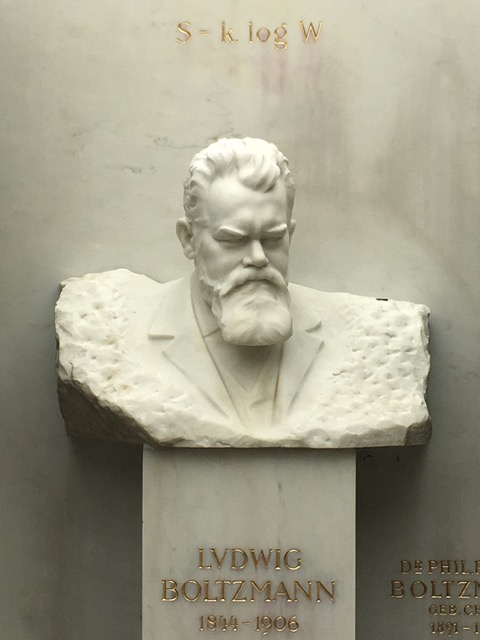
\includegraphics[scale=0.2]{./Bilder/Boltzmann.jpeg}
\caption{\label{fig_Boltzmann}%
Der Grabstein von Ludwig Boltzmann auf dem Zentralfriedhof von Wien. Oben 
ist die Formel f\"ur die statistische Entropie erkennbar. (eigenes Bild)}
\end{SCfigure}

In strenger Form gilt diese Formel zun\"achst nur f\"ur eine mikrokanonische Gesamtheit, also
ein thermodynamisches System, das vollkommen isoliert von seiner Umgebung ist, bei dem insbesondere
auch kein Austausch von W\"armeenergie mit der Umgebung m\"oglich ist (d.h., dieses System hat
adiabatische W\"ande). Ein solches thermodynamischer System ist durch einen Satz von makroskopischen
Gr\"o\ss en charakterisiert: die Energie $E$, das Volumen $V$, die Stoffmenge $n = N/N_{\rm A}$, wobei 
$N$ die Anzahl der Teilchen in dem System und $N_{\rm A}$ die Avogadro-Konstante sind, sowie
eventuell weitere makroskopisch beobachtbare und kontrollierbare Gr\"o\ss en. Die Menge $\Omega(E,V,n)$ 
der Mikrozust\"ande, die mit diesen makroskopischen Gr\"o\ss en vertr\"aglichen sind, h\"angt nat\"urlich
von den vorgegebenen Parametern ab. 

In der klassischen Mechanik ist \glqq Anzahl der Mikrozust\"ande\grqq\ eigentlich nicht gut definiert. Zun\"achst
einmal handelt es sich bei festem $E,V,n$ um einen Unterraum im $6N$-dimensionalen Phasenraum der
klassischen Teilchen. Das Volumen dieses Unterraums, das als Ma\ss\ f\"ur die Anzahl der Zust\"ande dienen
k\"onnte, verschwindet jedoch f\"ur eine feste Energie $E$ (es handelt sich um eine Hyperfl\"ache im Phasenraum,
deren Dimension um 1 kleiner ist als die des Phasenraums selbst). Daher betrachtet man f\"ur die erlaubten
Energien $\epsilon$ meist ein Energieintervall, $\epsilon \in [E-\Delta E, E]$, bzw.\ die Vollkugel $\epsilon \leq E$.
Es zeigt sich, dass bei sehr vielen Teilchen ($N$ in der Gr\"o\ss enordnung der Avogadro-Zahl) hier kein
messbarer Unterschied besteht. Au\ss erdem m\"ussen zwei \glqq \"Uberreste\grqq\ der Quantentheorie ber\"ucksichtigt
werden: die Ununterscheidbarkeit der Teilchen -- dies f\"uhrt auf einen Faktor $1/N!$ f\"ur die Abz\"ahlung verschiedener
Mikrozust\"ande -- und die Tatsache, dass Zust\"ande im Phasenraum innerhalb eines Volumens von $h^{3N}$
($h$ die Planck'sche Konstante)
nicht aufl\"osbar sind, d.h., das Volumen im Phasenraum ist in Einheiten von $h^{3N}$ anzugeben. 
In der Quantentheorie sind die Zust\"ande diskret und sollten der Ununterscheidbarkeit Rechnung tragen, sodass
die Anzahl der Zust\"ande mit einer Energie kleiner als ein vorgegebener Wert $E$ wohl definiert ist.  

In der mikrokanonischen Gesamtheit haben alle erlaubten Zust\"ande dieselbe Wahrscheinlichkeit, sodass
$p_i=1/|\Omega|$ und somit die Shannon-Information
\begin{equation}
              S = - \sum_i p_i \ln p_i = \sum_i p_i \ln |\Omega| = \ln |\Omega|  
\end{equation}
ist. Bis auf die Boltzmann-Konstante $k_{\rm B}=1,380\,649 \cdot 10^{-23}\,{\rm J/K}$, 
die eher historische Gr\"unde hat, stimmt dies mit der Boltzmann-Entropie
\"uberein. Der Faktor $k_{\rm B}$ hat zwei Gr\"unde: Zum einen hat die Entropie in der Thermodynamik die
Dimension \glqq Energie/Temperatur\grqq\, also J/K, und zum anderen ist die Anzahl der Mikrozust\"ande so
immens gro\ss, dass man riesige Zahlen f\"ur $\ln |\Omega|$ erh\"alt. Damit diese Zahlen mit den in der Thermodynamik
vertrauten Gr\"o\ss en \"ubereinstimmen, ber\"ucksichtigt man den Faktor $k_{\rm B}$.

Zu Beginn dieses Kurztextes wurde behauptet, dass die Boltzmann-Entropie als \glqq Ma\ss\ f\"ur
Unordnung\grqq\ verstanden werden kann. Wenn man unter Ordnung \glqq jedes Ding befindet sich an seinem
Platz\grqq\ versteht, gibt es nur einen (oder wenige) geordnete Zust\"ande. Je mehr Dinge sich nicht
an ihrem Platz befinden, umso gr\"o\ss er ist die Unordnung, umso gr\"o\ss er wird aber auch die Anzahl 
der M\"oglichkeiten, die f\"ur einen ungeordneten Zustand bestehen. Die Unordnung ist umso gr\"o\ss er,
je l\"anger man suchen muss, um einen bestimmten Gegenstand zu finden, bzw.\ je mehr M\"oglichkeiten
es gibt, wo sich ein Gegenstand befinden kann. Die Entropie w\"achst typischerweise
mit der Temperatur und bei einer absoluten Temperatur $T=0$ gibt es in der Quantentheorie nur
einen Grundzustand. Daher ist die Entropie dort null. Je h\"oher die Temperatur wird, umso ungeordneter
wird die Bewegung der Teilchen in einem System. In diesem Sinne ist die obige Aussage zu verstehen.

\section{Die Entropie des idealen Gases}

Ein Teil der gro\ss en Leistung von Ludwig Boltzmann bestand darin zu zeigen, dass die von ihm
angegebene Formel f\"ur die Entropie $S=k_{\rm B} \ln |\Omega|$ mit der thermodynamischen Entropie
\"ubereinstimmt. Konkret bewiesen hat er das f\"ur ein ideales Gas. Im Folgenden werden die Boltzmann-Entropie
sowie die thermodynamische Entropie eines idealen Gases auf verschiedenen Wegen hergeleitet. 

\subsection{Die thermodynamische Entropie eines idealem Gases}
\label{sec_Entropie_Therm}

In der Thermodynamik berechnet man die Entropie nach der Vorschrift von Sommerfeld
(siehe \hyperref[chap_zweiterHS]{Der zweite Hauptsatz der Thermodynamik}), indem man
die Gr\"o\ss e $\delta Q/T$ (W\"armemenge dividiert durch die
absolute Temperatur) entlang eines reversiblen Weges integriert, also
\begin{equation}
             S - S_0 = \int_0^1 \frac{\delta Q}{T} \, .
\end{equation}
Die W\"armemenge ist allgemein gegeben durch $\delta Q ={\rm d}E + p {\rm d}V$; dies ist
der Energiesatz -- der erste Hauptsatz der Thermodynamik -- f\"ur eine rein mechanische
Arbeit $\delta W = p{\rm d}V$. Speziell f\"ur ein ideals Gas gelten die kalorische Zustandsgleichung
$E= \frac{3}{2} n R T$ sowie die ideale Gasgleichung $pV=nRT$ ($n$ Stoffmenge in Mol,
$R= N_{\rm A}k_{\rm B} = 8,314\,462\,618\,153\,24\,{\rm J/(K\cdot mol)}$ ist die Gaskonstante mit der
Avogadro-Zahl $N_{\rm A}$), sodass
\begin{equation}
           \delta Q = \frac{3}{2} nR\, {\rm d}T + \frac{nRT}{V} {\rm d}V \, .
\end{equation}
Offenbar handelt es sich hierbei nicht um ein totales Differential, denn dann m\"usste
$\frac{\partial}{\partial V} \frac{3}{2}nR =0$ gleich $\frac{\partial}{\partial T} \frac{nRT}{V} =
\frac{nR}{V}$ sein, was offensichtlich nicht gilt, allerdings ist
\begin{equation}
           \frac{\delta Q}{T} = \frac{3}{2} \frac{nR}{T} {\rm d}T + \frac{nR}{V} {\rm d}V 
\end{equation}
ein totales Differential (wie es der zweite Hauptsatz auch fordert) und es gilt:
\begin{equation}
          S(T,V) = \int \frac{\delta Q}{T} = \int \frac{3}{2} \frac{nR}{T} {\rm d}T + \int \frac{nR}{V} {\rm d}V =
                \frac{3}{2} nR \ln \frac{T}{T_0} + nR \ln \frac{V}{V_0}  \, ,
\end{equation}
wobei $T_0$ und $V_0$ die Temperatur und das Volumen am Referenzpunkt $S_0$ sind. Dies ist
die gesuchte Funktion f\"ur die Entropie des idealen Gases. Allerdings war schon Gibbs bekannt, 
dass diese Gr\"o\ss e nicht additiv ist (d.h., wenn man das System verdoppelt, sodass sich $V$ und
$n$ verdoppeln, sollte sich auch $S$ verdoppeln). Wegen der Ununterscheidbarkeit der Teilchen 
muss man einen Term $N k_{\rm b} \ln N$ (wobei $N$ die Teilchenzahl ist) subtrahieren. 
Dies spielt an dieser Stelle aber keine Rolle. 

Um den Zusammenhang zur statistischen Herleitung der Entropie zu verdeutlichen, ersetzen
wir noch die Stoffmenge $n$ (in Mol) durch die Teilchenzahl $N= n N_{\rm A}$ und die Gaskonstante $R$
durch die Boltzmann-Konstante $R= N_{\rm A}k_{\rm B}$. Damit folgt f\"ur die Entropie:
\begin{equation}
\label{eq_Entropie_S}
          S(T,V) = \frac{3}{2} N k_{\rm B} \ln \frac{T}{T_0} + N k_{\rm B} \ln \frac{V}{V_0}  \, .
\end{equation}

\subsection{Die Entropie eines idealen Gases -- ein Skalenargument}

Die Entropie des idealen Gases Gl.\ \ref{eq_Entropie_S} l\"asst sich auch durch ein einfaches Skalenargument
nachvollziehen. Dazu betrachten wir zun\"achst die zu der Entropie geh\"orende \glqq Menge an 
Mikrozust\"anden\grqq\ im Sinne von Boltzmann:
\begin{equation}
\label{eq_Entropie_O}
           | \Omega | = \exp \left( \frac{S-S_0}{k_{\rm B}} \right) 
                     =  \left( \frac{T}{T_0} \right)^{\frac{3}{2}N} \left( \frac{V}{V_0} \right)^N                       
                     =  \left( \frac{E}{E_0} \right)^{\frac{3}{2}N} \left( \frac{V}{V_0} \right)^N      \, .
\end{equation}
Bei der zweiten Gleichung wurde ausgenutzt, dass die Energie eines idealen Gases nicht vom
Volumen abh\"angt und proportional zur Temperatur $T$ ist. Wir k\"onnen diese Abh\"angigkeiten
durch einfache Skalenargumente verstehen:
\begin{enumerate}
\item
Wenn wir das Volumen $V$ verdoppeln, verdoppelt sich f\"ur jedes Teilchen das Phasenraumvolumen,
d.h.\ wir erhalten einen Faktor $2^N$. Allgemeiner gilt: Wenn wir das Volumen um einen Faktor $\lambda$
skalieren, skalieren wir das Phasenraumvolumen pro Teilchen um denselben Faktor $\lambda$ und somit
das Phasenraumvolumen von $N$ Teilchen um den Faktor $\lambda^N$. Daher ist es naheliegend, dass
das Phasenraumvolumen von $N$ freien Teilchen proportional zu $V^N$ ist. 
\item
Wenn wir die Energie eines Teilchens verdoppeln, erh\"ohen wir jede seiner Impulskomponenten um 
$\sqrt{2}$, da die kinetische Energie -- nur diese gibt es bei einem idealen Gas -- proportional zu $p^2$ ist. 
Insgesamt erh\"oht sich das Phasenraumvolumen pro Teilchen um $2^{3/2}$, da ein Teilchen drei Impulskomponenten
hat. F\"ur $N$ Teilchen bedeutet dies einen Faktor $2^{3N/2}$. Allgemeiner: Wenn wir die Gesamtenergie
um einen Faktor $\lambda$ skalieren, skaliert das Phasenraumvolumen von $N$ Teilchen um den
Faktor $\lambda^{3N/2}$. Damit ist das Phasenraumvolumen von $N$ Teilchen proportional zu
$E^{3N/2}$.  
\end{enumerate}
Insgesamt folgt daher, dass sich f\"ur ein ideales Gas die Anzahl der Zust\"ande zu einer mittleren
Energie $E$ und einem Volumen $V$ wie $E^{3N/2} V^N$ verh\"alt. Da $|\Omega|$ eine dimensionslose
Zahl sein muss und sich diese \"Uberlegungen immer auf eine Referenzenergie $E_0$ und ein
Referenzvolumen $V_0$ beziehen, folgt Gl.\ \ref{eq_Entropie_O}. 

\subsection{Die quantenmechanische Herleitung der Boltzmann-Entropie\\eines idealen Gases}

Wir betrachten ein $N$-Teilchensystem in einem kubischen Kasten der Kantenl\"ange $L$, also 
vom Volumen $V=L^3$. Die quantenmechanischen Energiezust\"ande f\"ur ein freies Teilchen
in einem solchen Kasten sind
\begin{equation}
                   \epsilon_{n_1,n_2,n_3} = \frac{\hbar^2 \pi^2}{2 m L^2} (n_1^2 + n_2^2 + n_3^2)  \hspace{1cm}
                         n_i = 1, 2, ...\in \mathbb{N}  \, .
\end{equation}
F\"ur $N$ freie Teilchen sind die erlaubten Energiezust\"ande durch die Summe der Einteilchenenergien
gegeben:
\begin{equation}
                   \epsilon = \frac{\hbar^2 \pi^2}{2 m L^2} \sum_{i=1}^{3N} n_i^2 \, .
\end{equation}
Wir bestimmen zun\"achst die kumulative Anzahl $n(E,N)$ der Zust\"ande von $N$ freien Teilchen, 
sodass deren Energie kleiner oder gleich $E$ ist. Das f\"uhrt auf die Frage: Wie viele Kombinationen
von nat\"urlichen Zahlen $n_i$ gibt es, sodass $\sum_i^{3N} n_i^2 \leq R^2$ f\"ur eine vorgegebene
(gro\ss e) Zahl $R$? Wir l\"osen dieses Problem in zwei Schritten:
\begin{enumerate}
\item 
Wir bestimmen zun\"achst das Volumen einer $d$-dimensionalen Kugel.
\item
Wir l\"osen damit das genannte kombinatorische Problem.
\end{enumerate}
Schlie\ss lich betrachten wir f\"ur die Entropie nur die f\"uhrenden Terme.

\subsubsection{Das Volumen der $d$-dimensionalen Kugel}

Das Volumen einer $d$-dimensionalen Kugel vom Radius $R$ ist gegeben durch
\begin{equation}
        {\rm Vol}(R,d) = \int {\rm d} \Omega \int_0^R r^{d-1}{\rm d}r = \frac{1}{d}O(d) R^d \, , 
\end{equation}
wobei ${\rm d}\Omega$ die Winkelintegration in $d$ Dimensionen bezeichnet und
$O(d)$ ist die Oberfl\"ache der Einheitskugel (Kugel vom Radius $R=1$). Diese
Oberfl\"ache bestimmen wir folgenderma\ss en: Wir berechnen das Integral
\begin{equation}
          \left( \int_{-\infty}^\infty {\rm e}^{-x^2} {\rm d}x \right)^d = \pi^{d/2}
\end{equation}
in Kugelkoordinaten. Dort gilt
\begin{equation}
          \left( \int_{-\infty}^\infty {\rm e}^{-x^2} {\rm d}x \right)^d = 
          \int {\rm d}\Omega \int_0^\infty r^{d-1}{\rm e}^{-r^2} {\rm d}r  = \frac{1}{2} O(d) \Gamma (d/2) \, ,
\end{equation}
wobei die Definition der $\Gamma$-Funktion
\begin{equation}
      \int_0^\infty r^{d-1}{\rm e}^{-r^2} {\rm d}r  = \frac{1}{2} \int_0^\infty y^{d/2-1} {\rm e}^{-y}\,{\rm d}y = 
            \frac{1}{2}  \Gamma (d/2) 
\end{equation}
verwendet wurde. Aus diesen beiden Ergebnissen erhalten wir:
\begin{equation} 
\label{eq_Entropie_Od}
              O(d) = \frac{2 \pi^{d/2}}{\Gamma(d/2)} \hspace{0.8cm} \Rightarrow \hspace{0.8cm}
            {\rm Vol}(R,d) =  \frac{2}{d} \frac{\pi^{d/2}}{\Gamma(d/2)} R^d = \frac{\pi^{d/2}}{\Gamma(\frac{d}{2} + 1)} R^d  \, . 
\end{equation}

\subsubsection{Die Kombinatorik}

Die Bedingung $\sum_{i=1}^{3N} n_i^2 \leq R^2$ l\"asst sich folgenderma\ss en interpretieren: Gesucht ist
die Anzahl der Punkte
mit ganzzahligen, positiven Koordinaten $n_i$ innerhalb einer $3N$-dimensionalen Kugel vom Radius 
$R$. Da diese Punkte ein $3N$-dimensionales Gitter bilden und jede Gitterzelle das Volumen 1 hat,
k\"onnen wir die Frage in guter N\"aherung dadurch beantworten, dass wir das Volumen einer $3N$-dimensionalen
Kugel vom Radius $R$ betrachten.

Dieses Volumen ist durch Gl.\ \ref{eq_Entropie_Od} gegeben. Allerdings sind wir nicht an 
beliebigen ganzzahligen $3N$-Tupeln interessiert, sondern nur an den positiven. Da in dem Kugelvolumen jede 
Koordinate positive und negative Werte annehmen kann, erhalten wir das Volumen im rein positiven 
\glqq Quadranten\grqq, indem wir noch durch $2^{3N}$ dividieren. Au\ss erdem m\"ussen wir noch die
Ununterscheidbarkeit der Teilchen ber\"ucksichtigen, sodass wir noch durch $N!$ dividieren m\"ussen.
Die gesuchte Anzahl an Kombinationen $n(E,V,N)$ ist somit n\"aherungsweise:
\begin{equation}
                       n(E,V,N) = \frac{1}{2^{3N} N!} {\rm Vol}(R,3N)  \hspace{0.8cm} {\rm mit} \hspace{0.8cm}
                       R^2 = \frac{2 m L^2}{\hbar^2 \pi^2} E   \, .
\end{equation} 
Wir k\"onnten f\"ur das kombinatorische Problem nun noch Korrekturterme bestimmen, die sich daraus
ergeben, dass die Zahlen $n_i$ nicht 0 sein d\"urfen. F\"ur gro\ss e Werte von $R$, sodass Terme der
Ordnung $N/R$ vernachl\"assigt werden k\"onnen, spielen diese
Korrekturen jedoch keine Rolle. Als Ergebnis erhalten wir:
\begin{eqnarray}
\nonumber
               n(E,V,N) &=& \frac{1}{2^{3N} N!} \, 
               \left( \frac{2}{3N} \frac{\pi^{3N/2}}{\Gamma(3N/2)} \right)  \left( \frac{2 m L^2}{\hbar^2 \pi^2} E \right)^{3N/2} \\
\label{eq_Entropie_nEN}               
               &=& \frac{1}{N! \hbar^{3N}} \left( \frac{2}{3N} \frac{1}{\Gamma(3N/2)} \right)  \left( \frac{m}{2 \pi} E \right)^{3N/2}
                    V^N \, . 
\end{eqnarray}
Man erkennt an diesem Ergebnis schon die wesentlichen Elemente: (1) der Faktor $1/(N! h^{3N})$, der sich aus der
Quantentheorie ergibt (dass man den Phasenraum mit $h$ und nicht mit $\hbar$ normieren sollte, wird in
Abschnitt \ref{sec_Entropie_Kan} gezeigt), sowie (2) die Abh\"angigkeit $E^{3N/2} V^N$. 
  
\subsubsection{N\"aherungen}

In Abschnitt \ref{sec_Entropie_Therm} wurde erw\"ahnt, dass man zur thermodynamischen Entropie noch einen
Korrekturterm anbringen muss, um das Gibbs'sche Paradoxon zu vermeiden: Die Entropie sollte eine
additive Gr\"o\ss e sein, d.h., wenn sich die extensiven Gr\"o\ss en $E$ und $V$ verdoppeln, soll sich auch
die Entropie verdoppeln. Dazu betrachten wir die f\"uhrende $N$-Abh\"angigkeit vom Logarithmus von $n(E,N)$.

F\"ur die $\Gamma$-Funktion sowie den Term $N!$ verwenden wir die sogenannte Stirling'sche N\"aherung:
\begin{equation}
         N! \sim \sqrt{2 \pi N} \left( \frac{N}{\rm e} \right)^N \hspace{1cm} {\rm und} \hspace{1cm}
         \Gamma (x) \sim \sqrt{\frac{2\pi}{x}} \left( \frac{x}{\rm e} \right)^x  \, .
\end{equation}
Da wir letztendlich am Logarithmus von $n(E,N)$ interessiert sind und nur an der Abh\"angigkeit von 
$N$, $E$ und $V$, betrachten wir nur die Terme, die im Logarithmus proportional zu $N$ sind (alle anderen
Terme verschwinden f\"ur gro\ss e Werte von $N$ im Vergleich):
\begin{equation}
\label{eq_Entropie_Sn}
        \frac{S}{k_{\rm B}} = \ln n(E,V,N)  
        \approx  N \ln \left( \frac{E^{\frac{3}{2}} V}{N^{\frac{5}{2}}}C \right)  \hspace{1cm} {\rm mit} \hspace{1cm}  
        C = \frac{{\rm e}^{\frac{5}{2}}\, m^{\frac{3}{2}}}{(3\pi)^{\frac{3}{2}} \,\hbar^3} \, . 
\end{equation}
Die Konstante $C$ enth\"alt die Masse $m$ der Teilchen und $\hbar$ in einer Form, sodass
die Dimensionen stimmen, das Argument des Logarithmus also dimensionslos ist. 
Die anderen Konstanten wie $\pi$ und e sind f\"ur die Entropie nicht
relevant. Wichtig ist das Skalenverhalten von $S$ unter der Transformation $(E,V,N) \rightarrow
(\lambda E, \lambda V, \lambda N)$. Man erkennt, dass sich im Argument des Logarithmus 
alle Potenzen von $\lambda$
wegheben, sodass insgesamt von dem f\"uhrenden Faktor $N$ nur ein Faktor $\lambda$ auftritt, wie man es 
von der Entropie als extensiver Gr\"o\ss e auch erwartet. Ohne den Faktor $N!$ w\"are das nicht der Fall.

Man beachte, dass die Energie proportional zu $N$ ist, d.h., wenn wir die Energie \"uber die Beziehung
$E = \frac{3}{2} N k_{\rm B} T$ durch die absolute Temperatur $T$ ersetzen, erhalten wir im Logarithmus
die Kombination $T^{3/2}V/N$, die ebenfalls das richtige Skalenverhalten besitzt. $V/N$ ist das Volumen pro
Teilchen 

\subsection{Die Boltzmann-Entropie eines idealen Gases in der kanonischen\\Gesamtheit}
\label{sec_Entropie_Kan}

Abschlie\ss end bestimmen wir die freie Energie in der kanonischen Gesamtheit. Aus dieser
Gr\"o\ss e erhalten wir nicht nur unmittelbar die thermische Zustandsgleichung (also die ideale Gasgleichung
$p=p(V,T)$) sowie die kalorische Zustandsgleichung (die Beziehung zwischen der Energie und der Temperatur 
und dem Volumen, $E=E(V,T)$, wobei beim idealen Gas die Energie nicht vom Volumen abh\"angt) sondern
auch die Entropie des idealen Gases. 

\subsubsection{Die kanonische Zustandssumme}

Die kanonische Zustandssumme (einschlie\ss lich des Faktors $1/(N! h^{3N})$ aus der Quantentheorie -- man beachte, dass
hier die Planck'sche Konstante $h$ und nicht $\hbar$ steht) lautet in der klassischen N\"aherung:
\begin{equation}
     Z(T,V,N) = \frac{1}{N! h^{3N}} \int_{-\infty}^\infty \prod_i^{3N} {\rm d}p_i \int_{-\infty}^\infty \prod_i^{3N}{\rm d}x_i
          \exp \left( - \beta \sum_{i=1}^{3N} \frac{p_i^2}{2m} \right)  \, .
\end{equation} 
Die Integrale \"uber die Ortsfreiheitsgrade $x_i$ liefern insgesamt einen Beitrag $V^N$. Die Integrale \"uber
die Impulsfreiheitsgrade sind Gau\ss'sche Integrale und liefern f\"ur jeden Freiheitsgrad den Beitrag
\begin{equation}
            \int_{-\infty}^\infty {\rm d}p \exp  \left( - \frac{p^2}{2m k_{\rm B}T} \right) = \sqrt{2\pi m k_{\rm B}T} \, .
\end{equation}
Damit folgt insgesamt f\"ur die Zustandssumme $Z$ bzw.\ die freie Energie $F$:
\begin{equation}
        Z = \frac{1}{N! h^{3N}} V^N ( 2 \pi m k_{\rm B} T)^{3N/2} = \exp \left( - \frac{F}{k_{\rm B}T} \right)  \, .
\end{equation}

\subsubsection{Die kalorische Zustandsgleichung}

Aus der allgemeinen Darstellung der kanonischen Zustandssumme $Z= \sum_i {\rm e}^{-\beta E_i}$
erhalten wir f\"ur den Erwartungswert der Energie:
\begin{equation}
         \bar{E} = - \frac{\partial}{\partial \beta} \ln Z = \frac{1}{Z} \sum_i E_i {\rm e}^{-\beta E_i}
\end{equation} 
und damit f\"ur das ideale Gas die kalorische Zustandsgleichung: 
\begin{equation}
             \bar{E} = - \frac{\partial}{\partial \beta} \ln \beta^{-3N/2} =  \frac{3N}{2} \beta^{-1} = \frac{3N}{2} k_{\rm B}T \, .
\end{equation}

\subsubsection{Die thermische Zustandsgleichung -- Die ideale Gasgleichung}

Aus der allgemeinen Beziehung $\left( \frac{\partial}{\partial V}F\right)_{T,N} = - p$ erhalten wir die ideale
Gasgleichung: 
\begin{equation}
            p = \frac{\partial}{\partial V}\Big( k_{\rm B}T \ln V^N \Big) =  N k_{\rm B} T \frac{1}{V}
            \hspace{1cm} {\rm bzw.} \hspace{1cm}  p V = N k_{\rm B} T \, .
\end{equation}

\subsubsection{Die Entropie}

In der kanonischen Gesamtheit erh\"alt man die Entropie aus der Beziehung
\begin{equation}
              \left( \frac{\partial F}{\partial T} \right)_{V,N} = - S  \, .
\end{equation}
Mit $F = - k_{\rm B}T \ln Z $ folgt:
\begin{equation}
               S = k_{\rm B} \ln Z +  k_{\rm B} T \frac{\partial \ln Z}{\partial T} = k_{\rm B} \ln Z + k_{\rm B} \frac{3N}{2}  
\end{equation}
oder
\begin{equation}
              \frac{S}{k_{\rm B}} =   \ln Z +  \frac{3N}{2} \, . 
\end{equation}
In diesem Ausdruck betrachten wir wiederum nur die f\"uhrenden Terme der Stirling-Formel, wobei
der Term $\frac{3N}{2} = N \ln {\rm e}^{3/2}$ ber\"ucksichtigt wird:
\begin{equation}
           \ln Z  + \frac{3}{2}N \approx  N \ln \left( \frac{{\rm e}^{5/2} (2\pi m k_{B} T)^{3/2} V}{N h^3}  \right) 
\end{equation}
Ersetzen wir in dieser Formel die Temperatur $T$ durch die Energie $E$, also $k_{\rm B}T= \frac{2}{3} \frac{E}{N}$,
erhalten wir
\begin{equation}
          \frac{S}{k_{\rm B}}  \approx  N \ln \left( \frac{{\rm e}^{5/2} (4\pi m E)^{3/2} V}{N^{5/2} 3^{3/2} h^3}  \right) =
                      N \ln \left(  \frac{ E^{\frac{3}{2}} V}{N^{\frac{5}{2}}} C \right)
\end{equation}
mit
\begin{equation}
                C = \frac{{\rm e}^{\frac{5}{2}} (4\pi)^{\frac{3}{2}} m^{\frac{3}{2}}}{3^{\frac{3}{2}} h^3}  =
                       \frac{{\rm e}^{\frac{5}{2}} m^{\frac{3}{2}}}{(3\pi)^{\frac{3}{2}} \hbar^3}  \, .
\end{equation}
Wir erhalten somit exakt dasselbe Ergebnis wie aus der quantenmechanischen Berechnung, einschlie\ss lich
desselben Faktors $C$ aus Gl.\ \ref{eq_Entropie_Sn}. Man beachte, dass die beiden Konstanten $C$ nur
deshalb identisch sind, weil wir (1) die klassische Zustandssumme mit $1/h^{3N}$ normiert haben (und nicht mit
$1/\hbar^{3N}$) und weil wir bei der Berechnung der Entropie aus der freien Energie 
auch den konstanten Term $\frac{3}{2}N$ ber\"ucksichtigt haben.





\begin{thebibliography}{99}
\bibitem{Shannon} Shannon, C.\,E.; \textit{A Mathematical Theory of Communication}; Bell System Technical Journal.
             Short Hills N.J.\ (1948) 379--423 \& 623--656.     
\end{thebibliography}


\end{document}

